\documentclass[12pt]{jarticle}
\usepackage[dvipdfmx]{graphicx}
\usepackage{url}
\usepackage{listings,jlisting}
\usepackage{ascmac}
\usepackage{amsmath,amssymb}

%ここからソースコードの表示に関する設定
\lstset{
  basicstyle={\ttfamily},
  identifierstyle={\small},
  commentstyle={\smallitshape},
  keywordstyle={\small\bfseries},
  ndkeywordstyle={\small},
  stringstyle={\small\ttfamily},
  frame={tb},
  breaklines=true,
  columns=[l]{fullflexible},
  numbers=left,
  xrightmargin=0zw,
  xleftmargin=3zw,
  numberstyle={\scriptsize},
  stepnumber=1,
  numbersep=1zw,
  lineskip=-0.5ex
}
%ここまでソースコードの表示に関する設定

\title{知能プログラミング演習II 課題1}
\author{グループ8\\
  29114003 青山周平\\
}
\date{2019年10月15日}

\begin{document}
\maketitle

\paragraph{提出物} rep1, search.java, searchGUI.java
\paragraph{グループ} グループ8
\paragraph{メンバー}
\begin{tabular}{|c|c|c|}
  \hline
  学生番号&氏名&貢献度比率\\
  \hline\hline
  29114003&青山周平&NoData\\
  \hline
  29114060&後藤拓也&NoData\\
  \hline
  29114116&増田大輝&NoData\\
  \hline
  29114142&湯浅範子&NoData\\
  \hline
  29119016&小中祐希&NoData\\
  \hline
\end{tabular}



\section{課題の説明}
\begin{description}
\item[必須課題1-1]Search.javaの状態空間におけるパラメータ(コストや評価値)を様々に変化させて実行し,各探索手法の違いを説明せよ.
\hspace{4mm}具体的には,変化させたパラメータと探索結果(最短パス探索の成否,解を返すまでのステップ数,etc.)の関係を,探索手法毎に表やグラフ等にまとめよ.それらの結果を参照して考察を行い,各探索手法の違いを説明せよ. 
\item[必須課題1-2] グループでの進捗管理や成果物共有などについて,工夫した点や使ったツールについて考察せよ.
\item[発展課題1-3] Search.javaの探索過程や最終的に得られた順路をユーザに視覚的に示すGUIを作成せよ. 
\end{description}


\section{発展課題1-3}
\begin{screen}
Search.javaの探索過程や最終的に得られた順路をユーザに視覚的に示すGUIを作成せよ.
\end{screen}
私の担当箇所は,発展課題1-3のGUI全般のSwingを用いた実装である.

\subsection{手法}
GUIを実装するにあたり,以下のような方針を立てた.
\begin{enumerate}
\item 探索空間における各要素(ノードや経路)を表示する.
\item 要素に付随する値を入力するための入力ボックスを表示する.
\item 探索を選択するためのボタンと,実行ボタンを表示する.
\item 入力ボックスやボタンで入力した値をSearch.javaに反映し,実行する.
\item 得られた経路をGUIに反映する.
\end{enumerate}

1.に関して,ユーザーがなるべく直感的に理解できるようにすべく,表は用いずに1つの図の形式で完結するような仕様とした.

2.に関して,各要素とセットにして図中に入力ボックスを埋め込むことで,より直感的な入力を可能とした.また,入力ボックスには数値の入力に適したJSpinnerクラスを用いた.

3.に関して,探索の選択には,選択肢の表示に適したJRadiButtonクラスを用いた.値の反映にはActionListenerインターフェースを用いて,Search.javaの方も値を受け取って実行できるように改良した.

4.に関して,Search.javaから探索結果を渡すように改良し,受け取った結果を経路に再描写することで,ユーザーが視覚的に経路を得ることができる仕様とした.

\clearpage

\subsection{実装}

実装にあたり,主に下記のサイトを参考にした. \\

TATSUO IKURA: 『Swingを使ってみよう - Java GUIプログラミング』 https://www.javadrive.jp/tutorial/ (2019/10/15アクセス) \\

SearchGUI.javaには以下のクラスが含まれる.
\begin{itemize}
\item SearchGUI: メソッドmain, searchButtons, actionPerformedを実装したクラス
\item NodePanel: メソッドupdateと各種ゲッターを実装したノードに関するパネルを操作するためのクラス
\item PathPanel: メソッドpaintComponent, paintArrows, setShortestDistance, getMidPoints, execHor, execVer, update, forRepaintを実装した経路に関するパネルを操作するためのクラス
\end{itemize}

Search.javaは以下のように改良した.
\begin{itemize}
\item Searchクラスに,SearchGUI.java用の実行メソッドexecを追加.
\item Nodeクラスに,値の更新のためのメソッドsetHValue, remakeChildを追加.
\item Nodeクラスに値初期化のためのメソッドresetを追加.
\end{itemize}

\subsubsection{探索空間における各要素(ノードや経路)を表示するまで}
SearchGUIクラスではまず,フレームの中にmainPanelとsubPanelの2つのパネルを生成する.

mainPanelには経路やノードを格納するためのパネルを挿入した.ノードのパネルはJButtonクラスとJSpinnerクラスを用いて簡単にできるが,経路のパネルは線の描写が必要であるため,やや複雑なpaintComponentメソッドを拡張して用いる必要があった.

paintComponentの複雑な点は,このメソッドによって行われる描写は実行時に1度限りであるという点である.描写をパネルごとに分けて行いたかったので,その仕様は解決すべき課題となった.そこで経路のパネル用のクラスPathPanelを用意し,その中でpaintComponentメソッドを実装した.これによりインスタンスごとに描写呼び出しが行われて,経路を各パネルに分けることができた.

次に,表示についての課題が発生した.教科書通りのような経路図を表示するためには,各パネルを自由な位置に指定する必要があった.Swingには表を表示するのに適したレイアウトは数多くあるが,図を表示するためのレイアウトをあまり見つけることはできず,選択肢としては以下の2つの方法があった.
\begin{enumerate}
\item レイアウトマネージャーを無効にしてコンポーネントを座標指定で配置する.
\item SpringLayoutクラスを用いてコンポーネントを他のコンポーネントとの相対位置で指定して配置する.
\end{enumerate}

1.の方法のほうが簡単ではあるが,実行環境に依存するという問題があるため,2.の方法を用いて実装した.そうすると,経路の表示について,出発地と到着地のノードの座標から,その相対座標を計算する必要があった.そこで,getMidPointsメソッドではノードのパネル4面の各座標を計算し,setShortestDistanceメソッドを用いてノード間の最短距離を計算することで実装した.

getMidPointsメソッドをソースコード\ref{mid}に,
setShortestDistanceメソッドをソースコード\ref{dist}に示す.

\begin{lstlisting}[caption=getMidPointsメソッド, label=mid]
    Point[] getMidPoints(Rectangle r) {
        Point[] midPoints = new Point[4];
        for (int i = 0; i < midPoints.length; i++) {
            midPoints[i] = new Point();
        }
        midPoints[0].setLocation(r.x + r.width / 2.0, r.y); // 上の中点
        midPoints[1].setLocation(r.x + r.width, r.y + r.height / 2.0); // 右の中点
        midPoints[2].setLocation(r.x + r.width / 2.0, r.y + r.height / 2.0); // 下の中点
        midPoints[3].setLocation(r.x, r.y + r.height / 2.0); // 左の中点
        return midPoints;
    }
\end{lstlisting}

\begin{lstlisting}[caption=setShortestDistanceメソッド, label=dist]
    void setShortestDistance(Rectangle source, Rectangle distance) {
        Point[] fromMidPoints = getMidPoints(source);
        Point[] toMidPoints = getMidPoints(distance);

        double min = Double.MAX_VALUE;
        for (int i = 0; i < 4; i++) {
            Point from = fromMidPoints[i].getLocation();
            for (int j = 0; j < 4; j++) {
                Point to = toMidPoints[j].getLocation();
                double value = (from.getX() - to.getX()) * (from.getX() - to.getX())
                        + (from.getY() - to.getY()) * (from.getY() - to.getY());
                if (value < min) {
                    min = value;
                    start = from;
                    end = to;
                }
            }
        }
    }
\end{lstlisting}

次に,経路のパネルに,コストを格納するためのパネルを埋め込むためには,親となるパネルを大きめにする必要がある.そこで,int型のフィールドgraceを作り,相対座標にこの値を考慮することで,パネルの大きさに余裕を持たせることができた.

\subsubsection{要素に付随する値を入力するための入力ボックスを表示するまで}
まず,経路の初期値を得るためにSearch.javaを実行し,得られたノードを以下のようなMapで管理した.

\begin{lstlisting}[caption=mainメソッドの一部, label=map]
        for (int i = 0; i < 10; i++) {
            map.put(node[i], new NodePanel(node[i]));
        }
\end{lstlisting}

NodePanelクラスにおいて,これのインスタンスを親のパネルとし,ノードのラベルと値を格納するための入力ボックスを配置した.レイアウトには2行1列のGridLayoutクラスを利用した.
NodePanelのコンストラクタをソースコード\ref{node}に示す.

\begin{lstlisting}[caption=NodePanelのコンストラクタ, label=node]
    NodePanel(Node node) {
        id = counter++;
        this.node = node;
        setLayout(new GridLayout(2, 1));
        setBackground(Color.ORANGE);
        setBorder(new BevelBorder(BevelBorder.RAISED));

        JLabel label = new JLabel(id + ": " + node.getName());
        model = new SpinnerNumberModel(node.getHValue(), 0, 9999, 1);
        JSpinner spinner = new JSpinner(model);
        spinner.setPreferredSize(new Dimension(50, 25));

        add(label);
        add(spinner);
    }
\end{lstlisting}

\subsubsection{探索を選択するためのボタンと,実行ボタンを表示するまで}
探索を選択するためのボタンにはJRadioButtonクラスを用いた.複数選択を許可しないために,ButtonGroupクラスを用いた.
これらと実行ボタンを含んだパネルを生成するsearchButtonsメソッドをソースコード\ref{select}に示す.

\begin{lstlisting}[caption=searchButtonsメソッド, label=select]
    JPanel searchButtons() {
        JPanel p = new JPanel();
        p.setLayout(new BoxLayout(p, BoxLayout.PAGE_AXIS));
    
        radio = new JRadioButton[6];
        radio[0] = new JRadioButton("幅優先探索");
        radio[1] = new JRadioButton("深さ優先探索");
        radio[2] = new JRadioButton("分岐限定法");
        radio[3] = new JRadioButton("山登り法");
        radio[4] = new JRadioButton("最良優先探索");
        radio[5] = new JRadioButton("A*アルゴリズム");
        ButtonGroup group = new ButtonGroup();
        for (int i = 0; i < radio.length; i++) {
            group.add(radio[i]);
            p.add(radio[i]);
        }
        
        JButton button = new JButton("実行");
        button.addActionListener(this);
        p.add(button);

        return p;
    }
\end{lstlisting}

\subsubsection{入力ボックスやボタンで入力した値をSearch.javaに反映し,実行するまで}
まず,search.javaを反映した値を用いて再実行するために,再実行用のメソッドexecを実装した.

次に,実行ボタンを押したときに入力した値を反映するためには,ActionListenerインターフェースのactionPerformedメソッドを実装する必要がある.ノードの値,探索の種類,コストの値を全て反映し実行する,
actionPerformedメソッドの前半をソースコード\ref{act1}に示す.

\begin{lstlisting}[caption=actionPerformedメソッドの前半, label=act1]
    public void actionPerformed(ActionEvent e) {
        for (NodePanel p : map.values()) {
            p.getNode().reset();
            p.update((Integer)p.getModel().getValue()); // ヒューリスティック値の変更を反映
        }

        for (int i = 0 ; i < radio.length; i++){ // 探索の選択
            if (radio[i].isSelected()){
              which = i + 1;
            }
        }

        for(int i = 0; i < paths.size(); i++) {
            PathPanel p = paths.get(i);
            p.update((Integer)p.getModel().getValue()); // コストの変更を反映
        }
        
        ArrayList<Node> route = search.exec(which); // 再実行
\end{lstlisting}

\subsubsection{得られた経路をGUIに反映するまで}
再描写にはrepaintメソッドを用いる必要がある.これにより,paintComponentメソッドの再度呼び出しが行われるため,描写の条件による分岐をpaintComponent側で用意する必要がある.そこでPathPanelクラス内にboolean型のフィールドpassを用意し,forRepaintメソッド内で状態を確認,更新することで必要な経路のみ色を変えるような仕様にすることができた.また,Search.javaのexecメソッドの戻り値を,通るノードのみ格納したリストし,それを用いることで以上の操作を容易にした.

得られた経路を反映する,
actionPerformedメソッドの後半をソースコード\ref{act2}に示す.

\begin{lstlisting}[caption=actionPerformedメソッドの後半, label=act2]
        for(int i = 0; i < paths.size(); i++) {
            PathPanel p = paths.get(i);
            for(int j = 0; j < route.size() - 1; j++) {
                if(p.forRepaint(route.get(j), route.get(j + 1))) {
                    break;
                }
            }
            p.repaint();
        }
    }
\end{lstlisting}

\clearpage
\subsection{実行例}
SearchGUIを実行したところ,以下のような画面が得られる.

\begin{figure}[!hbt]
  	\begin{center}
  		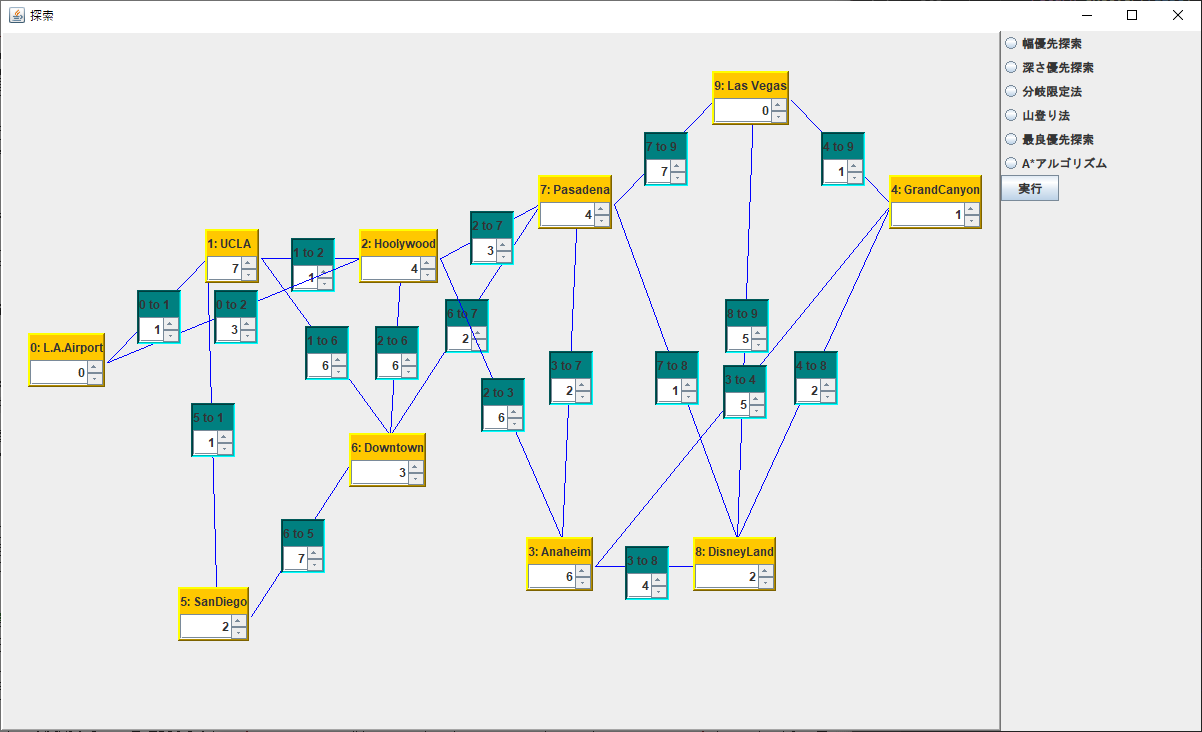
\includegraphics[scale=0.50]{scs1.png}
	\end{center}
  	\caption{初期状態}
\end{figure}
\clearpage

幅優先探索を選択し,実行したところ,以下のような画面が得られる.

\begin{figure}[!hbt]
  	\begin{center}
  		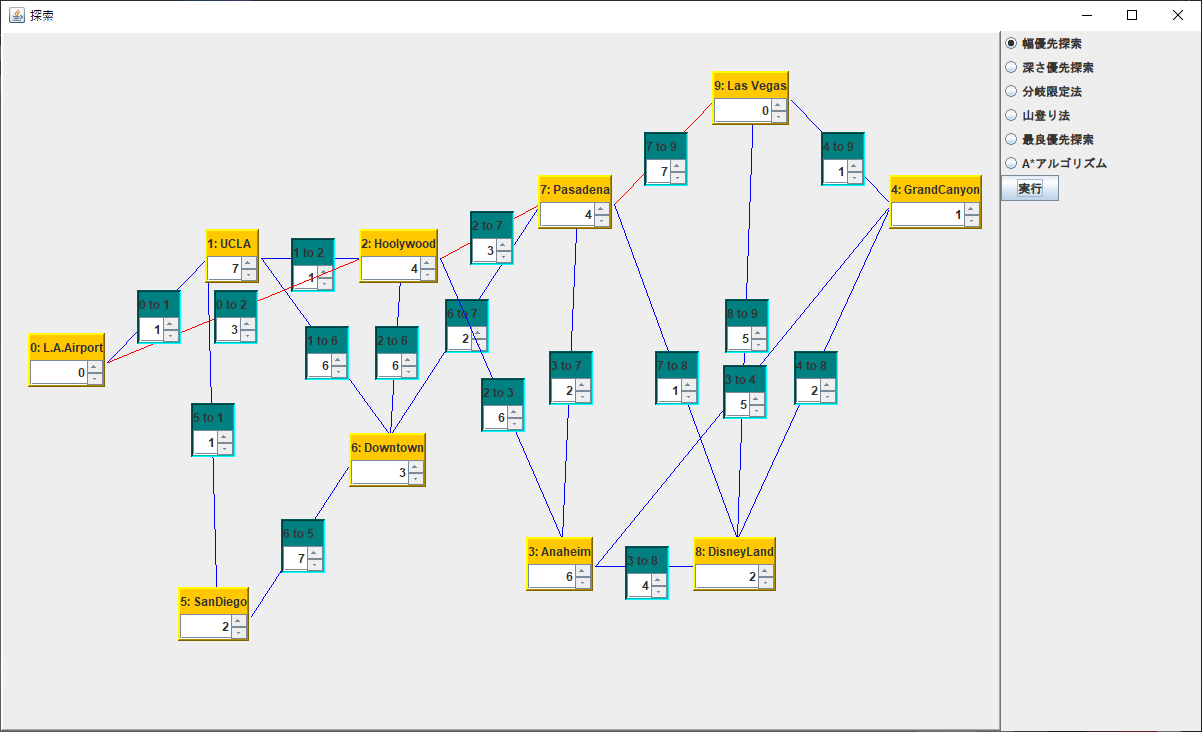
\includegraphics[scale=0.50]{scs2.png}
	\end{center}
  	\caption{幅優先探索の実行}
\end{figure}
\clearpage

同様にしてA*アルゴリズムを実行したところ,以下のような画面が得られる.

\begin{figure}[!hbt]
  	\begin{center}
  		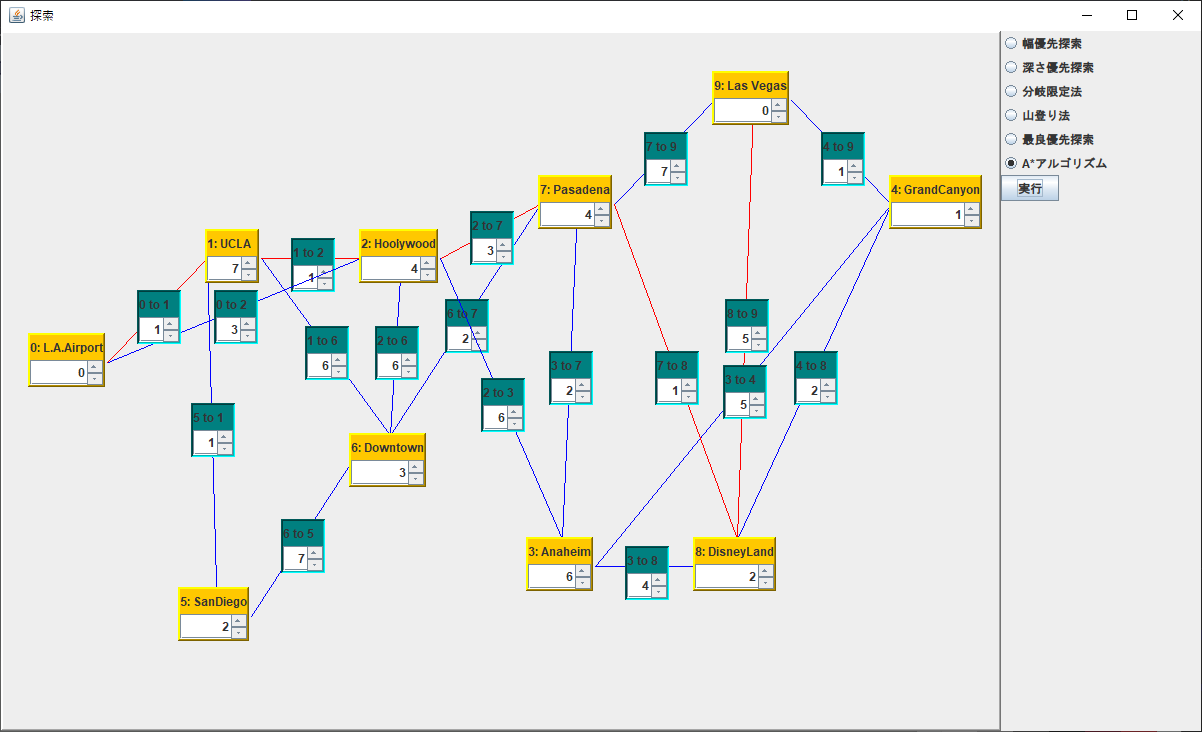
\includegraphics[scale=0.50]{scs3.png}
	\end{center}
  	\caption{A*アルゴリズムの実行}
\end{figure}
\clearpage

\subsection{考察}
初めてSwingを使ってみて,ボタンや入力ボックスを用いた表形式のGUIは作りやすそうだと感じた一方で,今回実装したような図形式のGUIは大変であると感じた.そもそも,SpringLayoutクラスによる相対座標の指定となると,実行と表示を繰り返しながら試行的に作っていかねばならず,また,相対座標というもの自体,パネルを階層的に作っている中で,正しく相対すべき相手との座標になっているかなどの点で間違いやすいと感じた.

一方で,マウスを使ったパネルの操作から,座標の取得もできるようなので,あらかじめそういったプログラムを作り,それによる座標の取得と保持を上手に実装できれば,Swingにおける自由な配置でのGUI制作も,より簡単なものになると考えられる.

また,表示面では,paintComponentメソッドの扱いも難しかった.関連する情報の載っているサイトがあまり見つからず,どのように扱えばよいのか理解するのに時間を要した.このメソッドは実行時に自動的に1度だけ呼び出されることが難点だと感じたが,インスタンスごとにこのメソッドを持たせることで,より自由で部分的な実行を可能にすることができた.このように,制約のあるものは,大元から変えてあげることや,javaであるならばオブジェクト指向を用いた分解ができないかを第一に考えることこそが,より迅速な問題解決につながると考えられる.

また,経路の表示には矢印を用いるよう試みたが,先述した相対座標の難しさ等もあり,上手に表示できなかったため断念した.また,矢印では先端部分の重なり等の問題等もあるため,今回のように"0 to 2"のようなラベルで表現した方が,誤解を減らす上でも役立ったと考えられる.しかし,経路同士の重なりを防ぐことはできないため,より誤解を減らすための方法として,線を曲線にすることや,線を縁取ることでより誤解の少ない表示ができるのではないかと考えられる.

また,今回NodePanelやPathPanelといったクラスに分解したことで,SearchGUIクラスのコードの複雑さを軽減することができた.これらのクラスは,実装中に分解できるんじゃないかと思い,後で分解したものであったので,今後はコードを書く前からクラスやメソッドとして取り出せないかを考えるようにすれば,より効率的なオブジェクト指向におけるプログラミングが見込めると考えられる.

Swingにおけるパネルについても,どこを一纏めにするかを予め考慮しておくことで,混乱せずにGUIの実装が見込めると考えられる.

\section{感想}
GUIのについては,警戒していたよりも簡単に実装することができた.ただ,線の描写や相対座標という概念には本当に苦しめられた.

最近,Unityを触っているが,あれを使えば今回のようなプログラムなどより簡単に,更に綺麗に作れるんじゃないかと終わった今感じている.そもそも,Swing自体こういった自由な配置のGUI作成には向いていないんじゃないかと感じ,実装しづらいもので頑張って実装しても見返りはあまりは大きくないな,と感じた.

それよりも,実装しやすいような形式に問題自体を変えられないか,目的の実装により向いているライブラリやソフトは無いか,ということを今後は軸に考えるようにしてゆきたい.これからは,いかに手を抜いて高品質なものを作れるかということを軸に取り組んでゆきたい.

\end{document}